% The WAA paper: the one document of Part 1 (the wet antenna equation), restructured on 2 November 2026 into a two-column
% academic paper (REVTeX 4-2, reprint style), modelled on docs/reference/Pulsed_NMR_Haber_Tsitseluk.pdf. The previous version
% is kept as docs/WAA_research_overview_v1.tex. What changed and the number check: research/wet_antenna/outputs/reports/overview_v2.md.
% Every number comes from research/wet_antenna/outputs (reports, tables, products/waa_equation_final.json) and
% research/baseline/outputs/reports. Figures: WAA_research_overview_figures/v2_*.png, made by figs_v2.py from saved tables only.
% Build: python docs/build_research_log.py WAA_research_overview   (writes docs/WAA_research_overview.pdf)
\documentclass[reprint,aps,pra,amsmath,amssymb,nofootinbib,superscriptaddress]{revtex4-2}
\usepackage[T1]{fontenc}
\usepackage[utf8]{inputenc}
\usepackage{lmodern}
\usepackage{graphicx}
\usepackage{booktabs}
\usepackage{tabularx}
\usepackage{array}
\usepackage{dcolumn}
\usepackage{microtype}
\usepackage{xcolor}
\definecolor{linkblue}{RGB}{26,54,104}
\usepackage[colorlinks=true,linkcolor=linkblue,citecolor=linkblue,urlcolor=linkblue]{hyperref}
\graphicspath{{WAA_research_overview_figures/}}

\renewcommand{\thesection}{\arabic{section}}
\renewcommand{\thesubsection}{\thesection.\arabic{subsection}}
\renewcommand{\thesubsubsection}{\thesubsection.\arabic{subsubsection}}
\makeatletter
\renewcommand{\p@subsection}{}
\renewcommand{\p@subsubsection}{}
\makeatother

\newcommand{\Rb}{\bar{R}}
\newcommand{\alink}{a_{\mathrm{link}}}
\newcommand{\Aband}{A_{\mathrm{band}}}
\newcommand{\cband}{c_{\mathrm{band}}}
\newcommand{\Fband}{F_{\mathrm{band}}}
\newcommand{\twet}{\tau_{\mathrm{wet}}}
\newcommand{\tdry}{\tau_{\mathrm{dry}}}
\newcommand{\iv}[2]{\,[#1,\,#2]}
\newcolumntype{L}{>{\raggedright\arraybackslash}X}

\begin{document}

\title{Wet antenna attenuation in commercial microwave links:\\ a dynamic law identified from data}

\author{Yonatan Haber}
\author{Yehonatan Tsitseluk}
\affiliation{CellEnMon lab, Tel Aviv University}
\date{November 2026}

\begin{abstract}
Commercial microwave links can measure rain, but a film of water on the antenna covers adds an attenuation that is not
caused by rain on the path. This wet antenna attenuation (WAA) is largest, relative to the signal, on short links, and it
is often removed with a constant correction or by subtracting an assumed rain law. We identify a dynamic WAA law from the
OpenMRG data of Gothenburg without subtracting any rain law. The antenna part and the path part are separated by their
different dependence on the link length, and the WAA alone is measured in the minutes after rain when the radar sees no
rain on the path. The resulting equation is a fast and a slow water store driven by the rain rate, $dW_f/dt = (0.72\,u -
W_f)/\tau_f$ with $\tau_f = 2.6$ min while wetting and 10.3 min while drying, a slow store with 240 min, a target $u =
\alink \Aband (R/5\ \mathrm{mm/h})^{0.54}$, and a path loss $L\,\cband R$. On 18 held-out storms, read once after a hashed
freeze, the equation predicts the attenuation better than no WAA, a constant WAA, a WAA without memory, the two published
WAA models with their default parameters and the refitted published model without memory, and as well as the refitted
published model with memory. Of all models with a link factor it is the only one whose link factor does not change with
the link length. Its main limit is the WAA level in light rain, which on the held-out storms is 0.4 to 0.6 dB higher than
the equation predicts.
\end{abstract}

\maketitle

% =====================================================================================================================
\section{Introduction}

Mobile networks connect their towers with point-to-point radio links, called commercial microwave links (CMLs). Each link
is a beam between two dish antennas, typically a few kilometres apart, at tens of GHz. The radios record the transmitted
and the received signal level, TSL and RSL in dBm, and their difference is the attenuation along the path. Raindrops
absorb and scatter microwaves, so the attenuation rises when it rains on the path, and the dense existing networks can
serve as rain sensors \cite{messer2006}. The measured attenuation, after the dry reference level (the baseline) is
removed, is written as
\begin{equation}
A(t) = \mathrm{TSL}(t) - \mathrm{RSL}(t) - B = A_{\mathrm{rain}}(t) + \delta(t),
\label{eq:A}
\end{equation}
where $B$ is the baseline and $\delta(t)$ collects every term that is not rain on the path. The rain term is a power law
integrated along the path,
\begin{equation}
A_{\mathrm{rain}}(t) = \int_0^L a\,R(x,t)^b\,dx \approx a\,\Rb(t)^b\,L,
\label{eq:powerlaw}
\end{equation}
with $R$ the rain rate in mm/h, $\Rb$ its mean along the path, $L$ the link length in km, and $a$ and $b$ coefficients
that depend on frequency and polarisation \cite{itu838}. The approximation is exact only for uniform rain.

Rain also wets the covers of the two antennas (the radomes), and a water film on a radome attenuates the signal. This
wet antenna attenuation, written $W$ in dB, is the main part of $\delta(t)$ during rain. It is local to the antennas,
so it does not grow with $L$, and it has memory, because the film builds up after rain starts and dries after rain
stops. On a short link the path term is small, so the same $W$ is a large share of $A$. A rain estimate that ignores
$W$ overestimates the rain, most strongly on short links \cite{leijnse2008}, and an antenna that is still wet after
the rain makes the link report rain that has already ended. Figure~\ref{fig:example} shows one storm on a 0.36 km and on a 4.13 km link.

\begin{figure}[t]
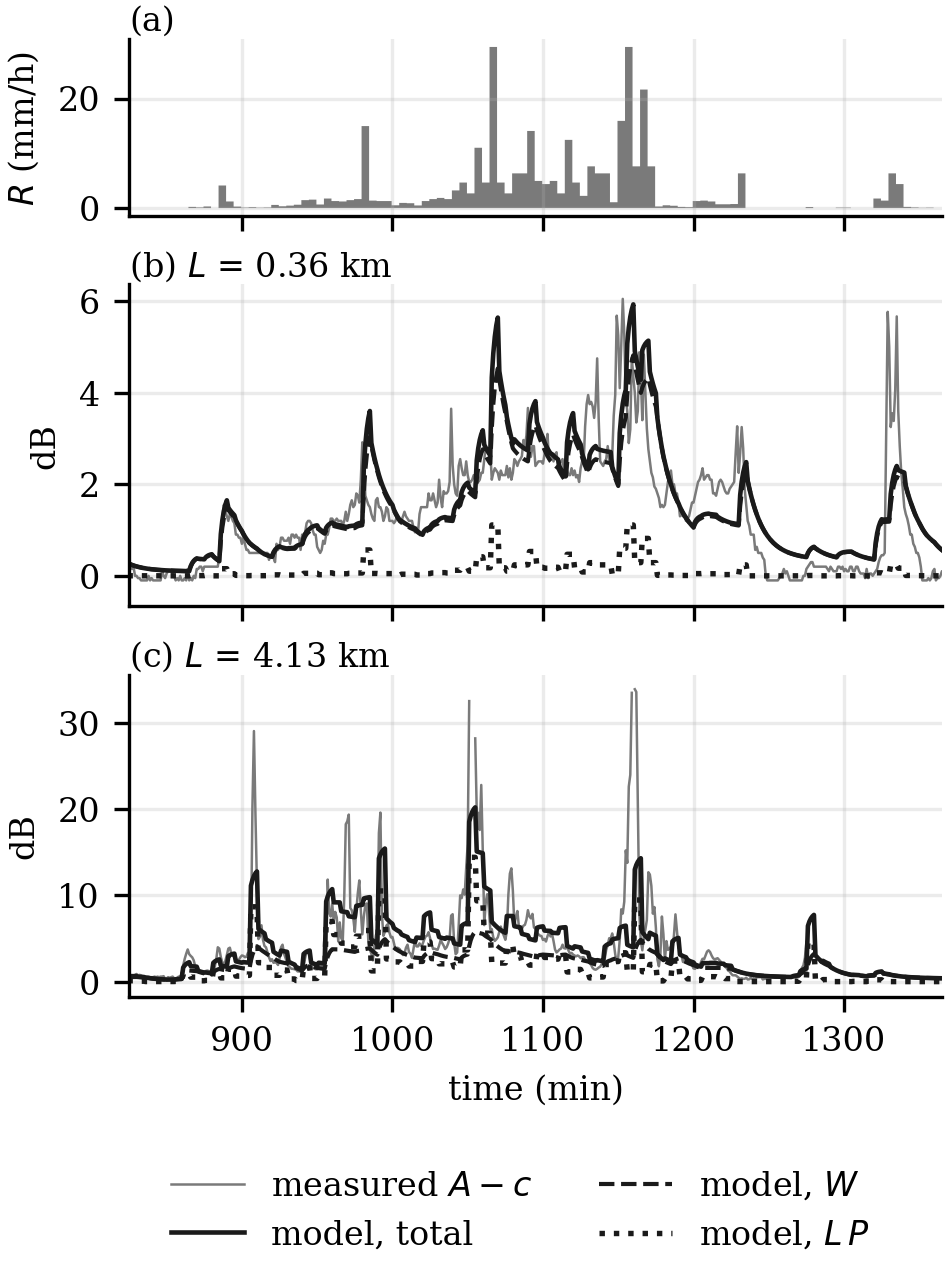
\includegraphics[width=\columnwidth]{v2_example_event.png}
\caption{One training storm on a short and a long 28 GHz link, one value per minute. (a) Rain over the short link.
(b), (c) Measured attenuation $A - c$ (thin grey line) and the model of Sec.~\ref{sec:eq}: total (solid), its antenna
part $W$ (dashed) and its path part $L\,P$ (dotted). On the short link the antenna part is most of the signal.}
\label{fig:example}
\end{figure}

Existing WAA models are of two kinds. Schleiss \emph{et al.}~\cite{schleiss2013} describe a WAA that rises toward a
maximum while it rains and decreases exponentially after the rain, measured on one experimental link. Pastorek
\emph{et al.}~\cite{pastorek2022} compared practical corrections, among them a WAA that depends on the rain rate
directly and has no memory. Direct measurements of the radome in the ATTRRA2 experiment showed that the real dynamics
can be more complex than these models \cite{tiede2023}, and laboratory measurements showed water running off a radome
directly after wetting \cite{tiede2025}.

A tempting way to measure WAA is to subtract a power-law rain term, Eq.~(\ref{eq:powerlaw}), from $A$ and to call the
rest WAA. We do not do this. Every error of the assumed rain law would then be counted as WAA, and a constant WAA would
look like a path term $f = L + L_0$, so the later study of the path law (Part 2 of the project) would inherit the error.
The aim of this work is a readable, dynamic equation for $W(t)$ with the rain as input, found from real data in a way that
never assumes a rain law. The work contributes four things. First, a model-free length test that measures the antenna
and the path parts separately from the dependence on $L$. Second, a two-store WAA equation with wetting and drying times
measured with rain gauges, whose antenna level and path loss were learned as free curves before closed forms were chosen.
Third, three tests, which need no rain law, that the WAA does not depend on the link length. Fourth, one comparison of all
WAA models under one protocol on held-out storms, both in accuracy and in physical consistency.

% =====================================================================================================================
\section{Data and preprocessing}
\label{sec:data}

\subsection{OpenMRG}
We use OpenMRG, an open dataset from Gothenburg, Sweden, for 1 June to 31 August 2015 \cite{openmrg}. It contains 728
sub-links (364 links, each measured in both directions) sampled every 10 s, with the RSL quantised to 0.3 dB and the TSL to
1 dB, at 7.5 to 38.7 GHz. A weather radar gives one rain map every 5 min on a grid of about 2 km, and ten city gauges
measure the rain on the ground every minute. A data pipeline cleaned and synchronised the links, averaged them to 1 min
and 5 min values, and marked rain events and quality problems. We kept the 28, 32 and 38 GHz bands, which hold 660 of the
728 sub-links (91\,\%). The other 68 sub-links belong to links of 4 km or more, so their antenna part cannot be separated
from their path part by comparing lengths.

\subsection{Split and selection}
Whole rain events were assigned before any modelling to a training set (TRAIN) for fitting, a validation set (VAL) for
choosing between model versions, and a test set (TEST) for one final check. In addition 71 of the 364 links (20\,\%) were
held out as unseen links. A link-event, one sub-link during one event, was kept only if it had a baseline, rain on the
link, a good sub-link status, a stable offset (spread at most 0.3 dB) and no TSL step during the rain
(Table~\ref{tab:split}). Rain is rare. Of the TRAIN minutes, 12\,\% have a rain rate of 0.5 mm/h or more and 0.4\,\% have
10 mm/h or more, so every result above 10 mm/h rests on few data.

\begin{table}[b]
\caption{The split of the data. A link-event is one sub-link during one rain event. Two of the 53 TRAIN events hold no
usable link-event. The largest loss is the link-events without rain on the link.}
\label{tab:split}
\begin{ruledtabular}
\begin{tabular}{lrrl}
Set & Events & Link-events & Use\\
\hline
TRAIN & 53 & 9\,780 & fitting (206 links)\\
VAL & 18 & 3\,250 & choosing between versions\\
TEST & 18 & 3\,355 + 1\,010 & one check (+ 59 new links)\\
\end{tabular}
\end{ruledtabular}
\end{table}

\subsection{The rain input}
The model needs the rain along every path every minute. Only the radar covers every path, but its scale error differs
from storm to storm, while the gauges are accurate but measure at ten points. The two are combined: the radar gives where
and when it rains on a path, and the gauges give how much. For each event in which the gauges caught at least 1 mm per
gauge link, the radar is divided by one factor per event,
\begin{equation}
R(t) = \frac{R_{\mathrm{radar}}(t)}{g_e}, \qquad g_e = \frac{\text{radar rain in event } e}{\text{gauge rain in event } e},
\label{eq:ge}
\end{equation}
and $g_e = 1$ otherwise. Pooled over the events, the radar measured 0.89 times the gauge rain on TRAIN and 1.71 times on
VAL. Section~\ref{sec:indep} shows why this factor matters.

\subsection{The baseline}
For each event and sub-link the baseline is one constant, the median attenuation over the 5 min slots of the 24 h before
the event that radar and gauges mark as dry and that start at least 1 h after the last rain. On fake events placed in dry
periods, where the true WAA is zero, the baseline error had a median of 0.00 dB and 10th and 90th percentiles of $-0.21$
and $+0.22$ dB, and one hour after real rain the baseline was only 0.04 dB above that of a dry control
(Appendix~\ref{app:baseline}). The offset $c$ is the median of $A$ over the dry minutes 120 to 30 min before the first
rain on the link.

% =====================================================================================================================
\section{Method}
\label{sec:method}

\subsection{The decomposition}
During an event the measured attenuation of a link is written as
\begin{equation}
A(t) - c = W(t) + L\,P\big(R(t-d)\big),
\label{eq:frame}
\end{equation}
where $P(R)$ is the specific path attenuation in dB/km and $d$ a lag of whole minutes. Neither $W$ nor $P$ has a form
imposed in advance. Table~\ref{tab:assume} lists the assumptions, the physical reason for each, and where each is tested.
The path term $L\,P(R)$ uses the mean rain along the path. It is exact for any rain pattern when $P$ is linear in $R$,
because then $\int c\,R(x)\,dx = c\,L\,\Rb$, and the data show that $P$ is close to linear (Sec.~\ref{sec:eq}).

\begin{table}[t]
\caption{The assumptions of Eq.~(\ref{eq:frame}).}
\label{tab:assume}
\begin{tabularx}{\columnwidth}{LLL}
\toprule
Assumption & Physical reason & Tested in\\
\midrule
The two parts add & separate losses in series & length test, Sec.~\ref{sec:lt}\\
$W$ does not depend on $L$ & two antennas on every link & Sec.~\ref{sec:indep}\\
Path part is $L$ times a loss per km & equal rain, equal loss per km & quadratic term in 4 of 15 classes\\
$R_{\mathrm{radar}}/g_e$ is the rain & radar for where, gauges for how much & VAL gap closed, Sec.~\ref{sec:indep}\\
Rain drives the wetting & the water comes from rain & dew excluded, Sec.~\ref{sec:discussion}\\
\bottomrule
\end{tabularx}
\end{table}

\subsection{The length test}
\label{sec:lt}
For one link, Eq.~(\ref{eq:frame}) has two unknowns. The two parts, however, depend differently on the length. The
antenna part is the same on every link, while the path part grows with $L$. Between links of different length in the same
rain, a difference in $A - c$ therefore comes from the path. In practice we collect the 5 min values of steady rain whose
path rain falls in one class (0.5--1, 1--2, 2--5, 5--10 and 10--20 mm/h) from all links and events, take for each link and
event the median of $A - c$ in that class, and fit a robust (Huber) straight line
\begin{equation}
A - c = I + s\,L.
\label{eq:line}
\end{equation}
The intercept at $L = 0$ is the antenna part, $I = W$, and the slope is the loss per km, $s = P$. The 90\,\% intervals come
from resampling whole events (1000 draws). Each band and rain class (a cell) gives one point of the curves $W(R)$ and
$P(R)$, and a cell is used for a verdict only if it holds at least 8 links shorter than 1 km. No model enters this test.
The same line can also be fitted through a model's own predictions on the same 5 min values, which tells whether the model
splits $A$ the way the data do.

\subsection{Memory: a two-store model}
The water on a radome does not follow the rain instantly. We model it as a store that relaxes toward a target set by the
current rain,
\begin{equation}
\frac{dW}{dt} = \frac{u(t) - W}{\tau}, \qquad u(t) = \alink\,F\big(R(t-d)\big),
\label{eq:bucket}
\end{equation}
where $F(R)$ is the steady WAA in constant rain $R$ and $\alink$ a dimensionless factor per link (the link factor),
because some antennas collect more water than others. When $W$ is below its target the store fills (wetting), and when it
is above, it empties (drying). Wetting and drying have their own time constants, and a small part of the water stays for
hours, so the store is split into a fast part with a share $\varphi$ and a slow part,
\begin{align}
\frac{dW_f}{dt} &= \frac{\varphi\,u - W_f}{\tau_f}, \qquad
\tau_f = \begin{cases} \twet & \text{if } \varphi\,u > W_f\\ \tdry & \text{otherwise,}\end{cases}
\label{eq:fast}\\
\frac{dW_s}{dt} &= \frac{(1-\varphi)\,u - W_s}{\tau_s}, \qquad W = W_f + W_s.
\label{eq:slow}
\end{align}
For a step in the rain the fast store follows $\varphi u\,(1 - e^{-t/\twet})$ while wetting and $W_0\,e^{-t/\tdry}$ while
drying, with $W_0$ the water left when the rain stops. Figure~\ref{fig:memory} shows the response of the final equation to
one hour of steady rain.

The radar, with its 5 min maps, cannot resolve time constants of a few minutes. On fake data a 5 min noisy input alone made
the fitted wetting 2.1 times slower. The time constants and the share were therefore measured with the gauges, which
record the start and end of rain to the minute, and then held fixed in the radar fit.

\begin{figure}[t]
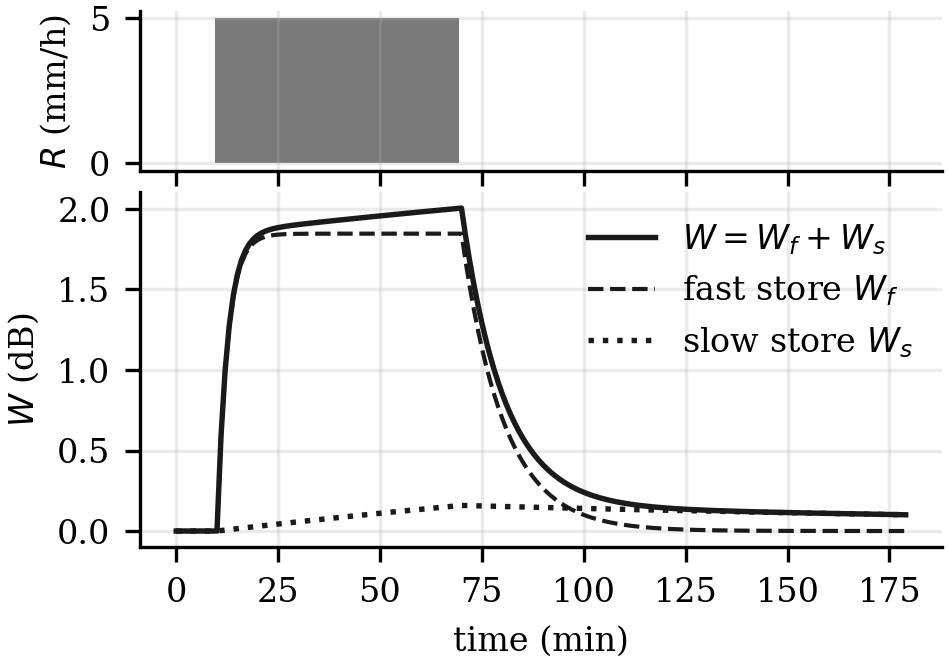
\includegraphics[width=\columnwidth]{v2_memory.png}
\caption{Response of the final equation (computed, not measured) to 60 min of 5 mm/h on a 28 GHz link with $\alink = 1$.
The fast store fills within minutes and empties within about 30 min, and the slow store remains for hours.}
\label{fig:memory}
\end{figure}

\subsection{Learning $F$ and $P$, then choosing closed forms}
All parts of Eqs.~(\ref{eq:frame})--(\ref{eq:slow}) were fitted together on TRAIN with $F$ and $P$ as free curves, that
is, values at fixed rain rates from 0.05 to 40 mm/h joined by straight lines. The loss is a Huber loss of the 5 min
residuals with a 0.3 dB threshold, and $\ln\alink$ carries a weak prior around zero, which fixes the product $\alink F$
but not the level of $F$ alone. Only after the free curves were known were closed forms fitted to them. Physical forms
(curves that saturate at a maximum, capped power laws) and forms proposed by symbolic regression with PySR
\cite{cranmer2023} competed under one rule, the corrected Akaike information criterion (AICc), which weighs the fit
against the number of parameters. The chosen form was put back into the full model, refitted, and accepted only if it
predicted unseen events as well as the free curve and still passed the length test.

\subsection{Validation protocol}
Every step followed the same protocol. The pass rule of a check was written down, dated, before the check was run. Every
fitted number was first recovered on fake data generated from the model with realistic noise on the real links and the
real rain. Intervals come from refitting on resampled sets of whole events. Structural choices were judged on VAL, never
on TRAIN alone, so numbers on VAL are optimistic. Before TEST was read, the equation, three simpler comparison models and
the pass rules were frozen and their cryptographic hashes committed, and TEST was then read once. A decision that
deviated from a written rule was dated and its reason recorded (Appendix~\ref{app:decisions}).

% =====================================================================================================================
\section{Results}
\label{sec:results}

\subsection{What the data say without a model}
\label{sec:modelfree}
Figure~\ref{fig:length} shows the length test on TRAIN. In each rain class the points of $A - c$ lie around a straight line
in $L$. The intercepts, the antenna part, rise from about 1.0 dB at 0.5 to 1 mm/h to 2.4 to 2.8 dB at 5 to 20 mm/h and then
grow only slowly, while the slopes, the path loss per km, grow roughly in proportion to $R$. A WAA that is constant in rain
would give a flat intercept, which the data exclude, and a WAA that grows with the path would show up as a slope that does
not follow the rain. The test also showed why short links alone are not enough. When all links are short, a small path loss
and a slightly larger antenna loss have nearly the same effect, and the fitted path loss on links below 1 km halved when
links up to 3 km were added. The model was therefore fitted on all lengths together.

\begin{figure}[t]
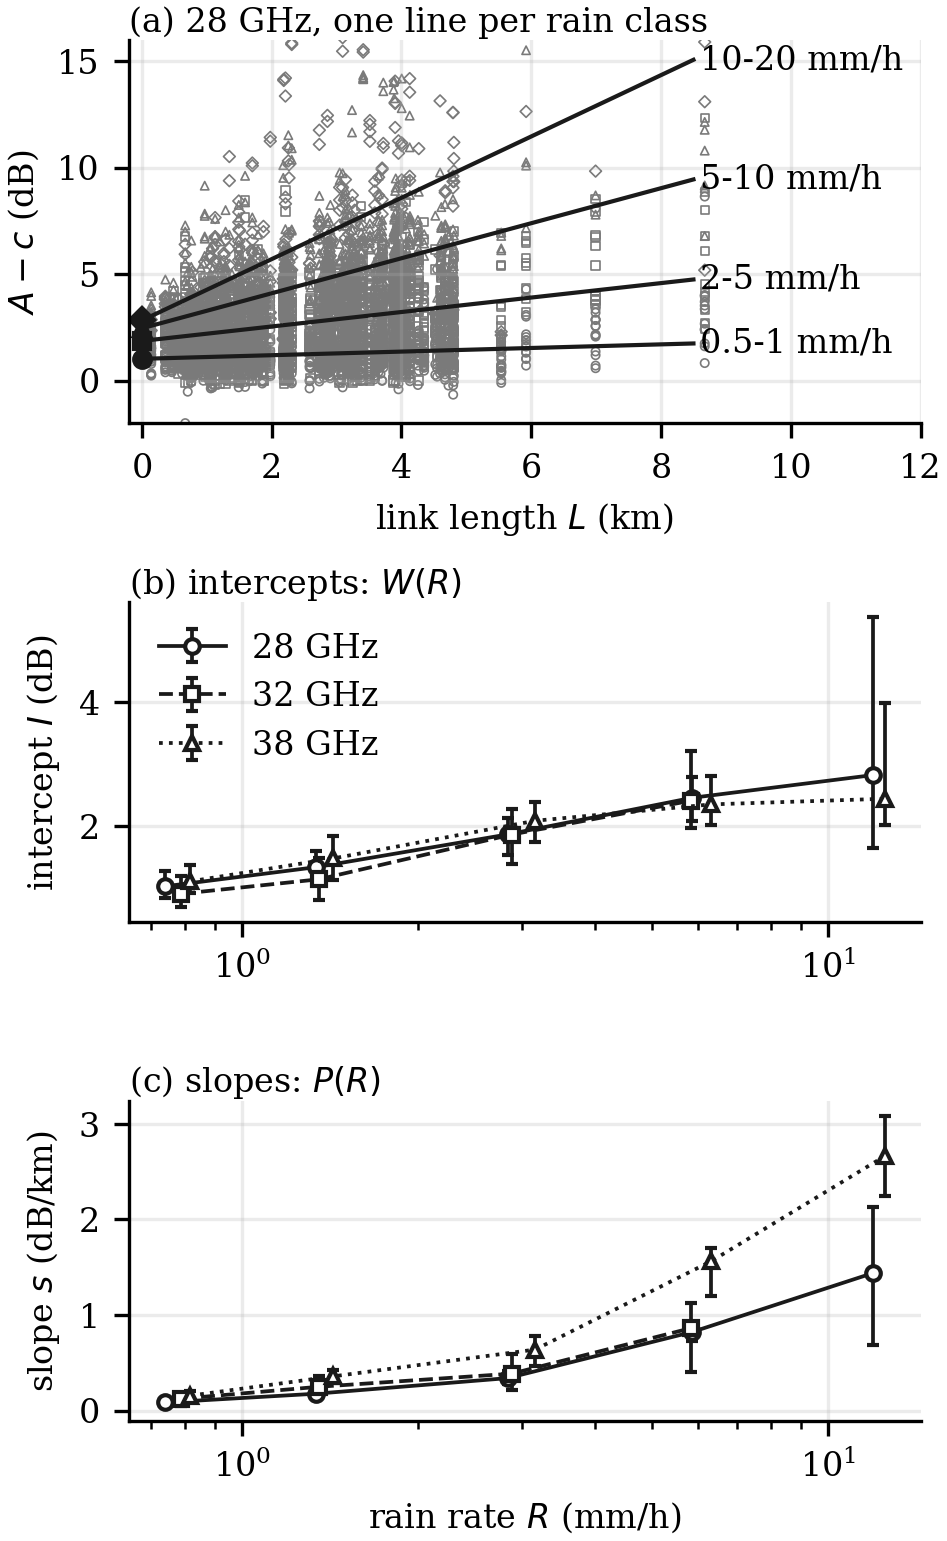
\includegraphics[width=\columnwidth]{v2_length_test.png}
\caption{The model-free length test on TRAIN. (a) Each point is one link in one event at 28 GHz, grouped by rain class
(marker shape), with the robust line of each class. (b) The intercepts at $L = 0$ give the antenna part $W(R)$. (c) The
slopes give the path attenuation per km $P(R)$. Bars are 90\,\% event-bootstrap intervals. Line style and marker show the
band.}
\label{fig:length}
\end{figure}

\subsection{The equation}
\label{sec:eq}
On the free curves, one shape of $F$ scaled by one level per band predicted VAL as well as separate shapes per band (RMSE
0.3875 against 0.3878 dB), although TRAIN alone favoured separate shapes. $F$ rises steeply in light rain and more slowly
above, and $P$ is close to linear in $R$ (Fig.~\ref{fig:FP}). The simplest closed form that describes $F$ as well as the
free curve is a power of $R$ close to a square root, proposed by PySR, and the linear form was chosen for $P$. The full
equation with all its numbers is given in Fig.~\ref{fig:model}. The exponent $b = 0.54$ has the interval 0.47 to 0.63,
which contains 0.5 and excludes a linear dependence. The formula has no maximum, so the data do not show whether WAA
saturates, and it is not valid above 40 mm/h.

\begin{figure*}[t]
\setlength{\fboxsep}{6pt}\setlength{\fboxrule}{0.6pt}%
\fbox{\begin{minipage}{0.97\textwidth}\small\setlength{\parindent}{0pt}
\textsc{Measured quantity.} $A(t) = \mathrm{TSL}(t) - \mathrm{RSL}(t) - B$ in dB at 1 min, $B$ the median dry attenuation of
the 24 h before the event (48 h if less than 1 h of dry data remains), $c$ the median of $A$ over the dry minutes 120 to
30 min before the first rain on the link (0 if fewer than 30 such minutes).
\textsc{Inputs.} Link length $L$ (km), band from the frequency, 28 GHz (25--30.5 GHz), 32 GHz (30.5--35 GHz), 38 GHz
(35--45 GHz), link factor $\alink$, and the rain $R(t) = R_{\mathrm{radar}}/g_e$ in mm/h, one value per minute, with
$R_{\mathrm{radar}}$ the radar rain averaged over the pixels along the path and held over its 5 min interval and $g_e$ the
ratio of radar to city-gauge rain of the event over the gauges within 1 km of a path ($g_e = 1$ if the gauges caught less
than 1 mm per gauge link).
\begin{align*}
A(t) - c &= W_f(t) + W_s(t) + L\,\cband\,R(t-d), &
u(t) &= \alink\,\Aband\left(\frac{R(t-d)}{5\ \mathrm{mm/h}}\right)^{b},\\
\frac{dW_f}{dt} &= \frac{\varphi\,u(t) - W_f}{\tau_f},\quad \tau_f = \begin{cases}\twet & \text{if } \varphi\,u > W_f\\ \tdry & \text{otherwise}\end{cases}, &
\frac{dW_s}{dt} &= \frac{(1-\varphi)\,u(t) - W_s}{\tau_s}.
\end{align*}
Initial state $W_f = W_s = 0$ in dry weather before the event. One step per minute, $W \leftarrow v + (W - v)\,e^{-1/\tau}$
with $v$ the target of the store, output after the step.

\smallskip
\begin{tabularx}{\linewidth}{@{}p{3.6cm} L p{6.2cm}@{}}
\toprule
Parameter & Value (90\,\% interval) & Source\\
\midrule
$A_{28}$, $A_{32}$, $A_{38}$ (dB) & 2.57\iv{2.00}{3.21}, 2.36\iv{1.70}{3.06}, 2.77\iv{2.25}{3.40} & fitted on TRAIN, 40 event-bootstrap refits\\
$b$ & 0.54\iv{0.47}{0.63} & fitted, as above\\
$c_{28}$, $c_{32}$, $c_{38}$ (dB km$^{-1}$ per mm/h) & 0.105\iv{0.058}{0.138}, 0.141\iv{0.047}{0.190}, 0.194\iv{0.111}{0.245} & fitted, as above\\
$\alink$ & one per TRAIN link (206 links), 10th to 90th percentile 0.77 to 1.24, 1 for a new link & fitted with the above\\
$\twet$, $\tdry$ (min) & 2.6\iv{2.4}{3.1}, 10.3\iv{9.2}{11.8} (VAL 2.0\iv{1.5}{3.2}, 8.8\iv{5.8}{13.1}) & fixed, from the gauge-input fit on TRAIN\\
$\varphi$ & 0.72\iv{0.60}{0.81} & fixed, as above\\
$\tau_s$ (min) & 240 & fixed at the search bound, not identified\\
$d$ (min) & 1 & selected in the fit\\
\bottomrule
\end{tabularx}

\smallskip
\textsc{Validity.} $0 \le R \le 40$ mm/h (above 10 mm/h based on 0.4\,\% of the minutes), the three bands, link lengths
0.14 to 8.7 km, OpenMRG (Gothenburg, summer 2015). Not identified: $\tau_s$ and $\varphi$, the path loss below 1 mm/h, and the
level of $F$ apart from $\alink$.
\end{minipage}}
\caption{The WAA equation of Part 1, frozen for the test, with the closed form of $F$ adopted after it
(Sec.~\ref{sec:rules}). All values and the per-link factors are stored in the equation file of the project and computed by
its reference implementation, which reproduces the fit to $10^{-15}$ dB.}
\label{fig:model}
\end{figure*}

\begin{figure}[t]
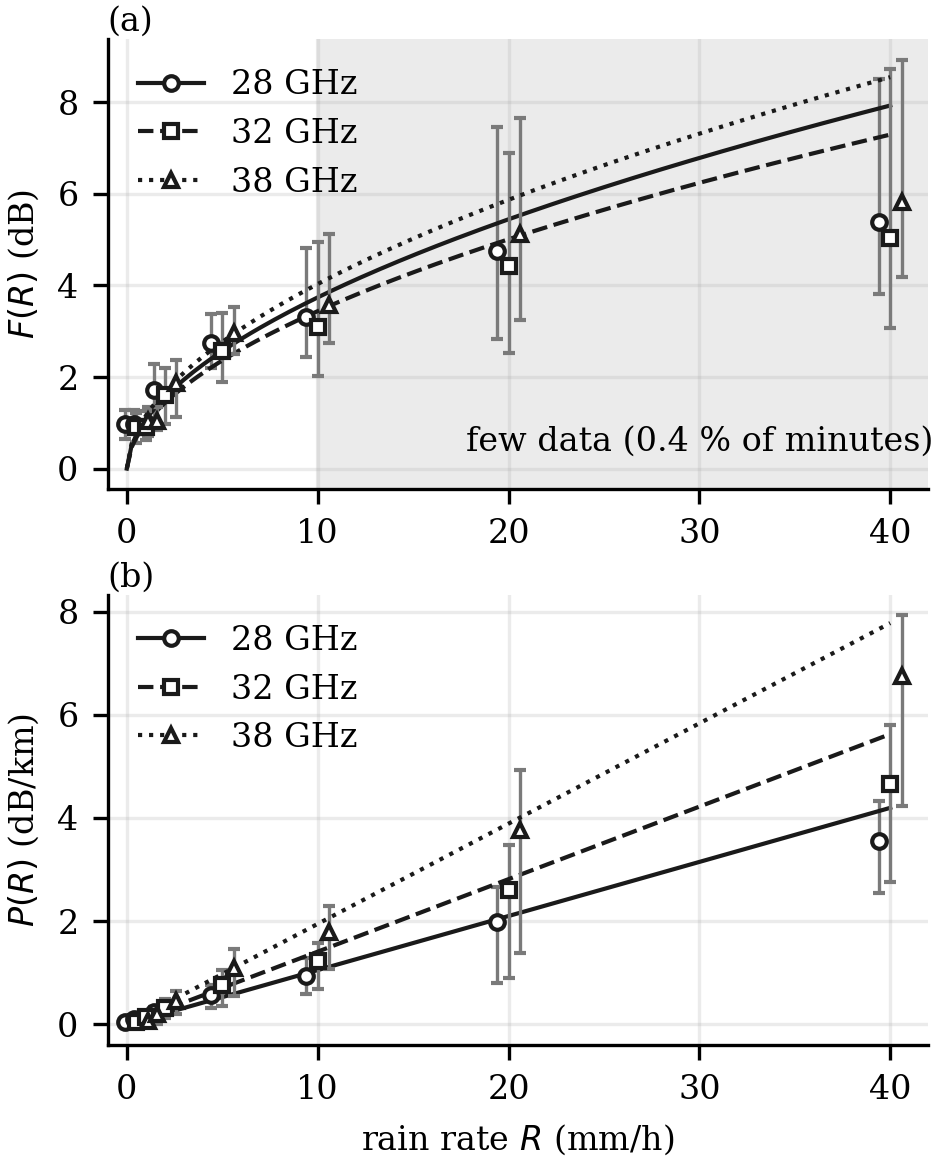
\includegraphics[width=\columnwidth]{v2_F_P.png}
\caption{The learned curves on TRAIN. Points: free curves with 90\,\% intervals. Lines: the closed forms, one line style per
band. (a) Steady WAA $F(R)$ and $\Aband (R/5)^{0.54}$. Above 10 mm/h (shaded) $F$ is poorly determined. (b) Path
attenuation per km $P(R)$ and $\cband R$.}
\label{fig:FP}
\end{figure}

All nine numbers of the closed form were recovered within 20\,\% on fake data, as were all 62 numbers of the free curves,
61 of them within 10\,\%. Eight numbers, the path loss below 1 mm/h, are too close to zero to be distinguished from it and
are not reported. The data fix the product $\alink F$. The level of $F$ alone is set by the weak prior that keeps the
median $\alink$ near 1.

\subsection{WAA does not depend on the link length}
\label{sec:indep}
The central assumption of Eq.~(\ref{eq:frame}) was tested in three ways that need no rain law, before TEST was read. First,
the link factor does not depend on the length (Fig.~\ref{fig:alink}). Its Spearman correlation with $L$ is $+0.05$
(interval $-0.07$ to $+0.17$) for the model frozen for the test and $+0.09$ ($-0.03$ to $+0.20$) for the final equation.
Second, the length test repeated with links shorter than 3 km only and with links longer than 1.5 km only gave the same
intercept in 13 of 15 cells. Third, in 9\,081 periods after rain, on 206 links in 23 TRAIN and 10 VAL events, the radar
showed no rain on any pixel of the path. There the path term is zero, so $A - c$ is the WAA alone, measured without any
model. The measured WAA and the model error were the same for short, medium and long links, with a median error of
$-0.18$ dB at 10 min in every length class (Fig.~\ref{fig:drypath}).

The same tests located the one large gap between TRAIN and VAL in the rain input, not in the antennas. With the raw radar
the VAL length test agreed in at most 1 of 8 cells, and with the gauge factor of Eq.~(\ref{eq:ge}) in 5 of 6. A
rate-dependent radar error, which would need a curve instead of one factor, was not found: its apparent dependence reversed
when the data were binned by the radar instead of the gauge, the signature of regression to the mean between two noisy
measurements.

\begin{figure}[t]
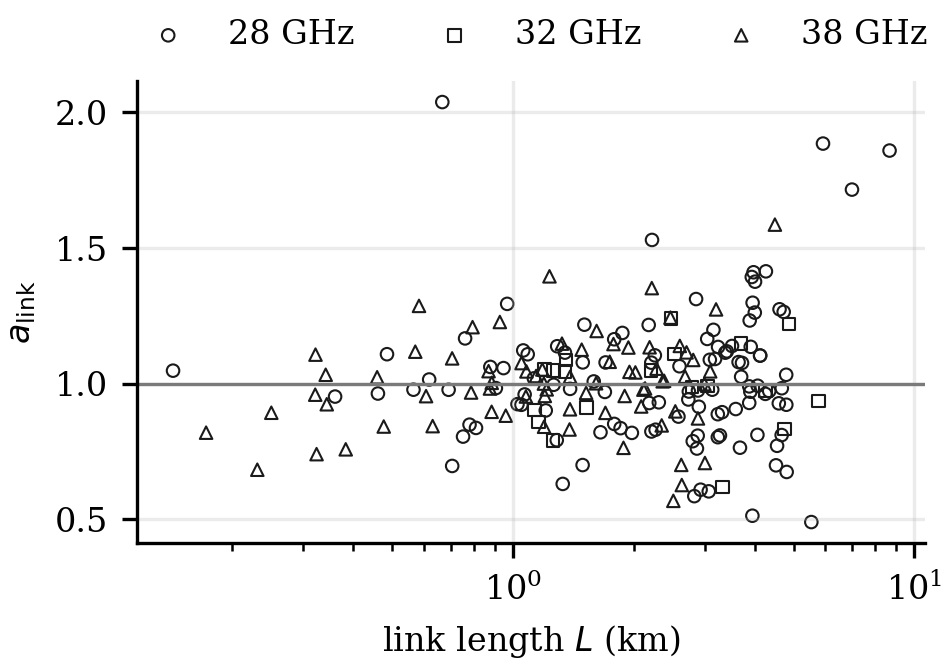
\includegraphics[width=\columnwidth]{v2_a_link.png}
\caption{The link factor $\alink$ of each of the 206 TRAIN links against its length. Marker shape gives the band. There is
no trend.}
\label{fig:alink}
\end{figure}

\begin{figure}[t]
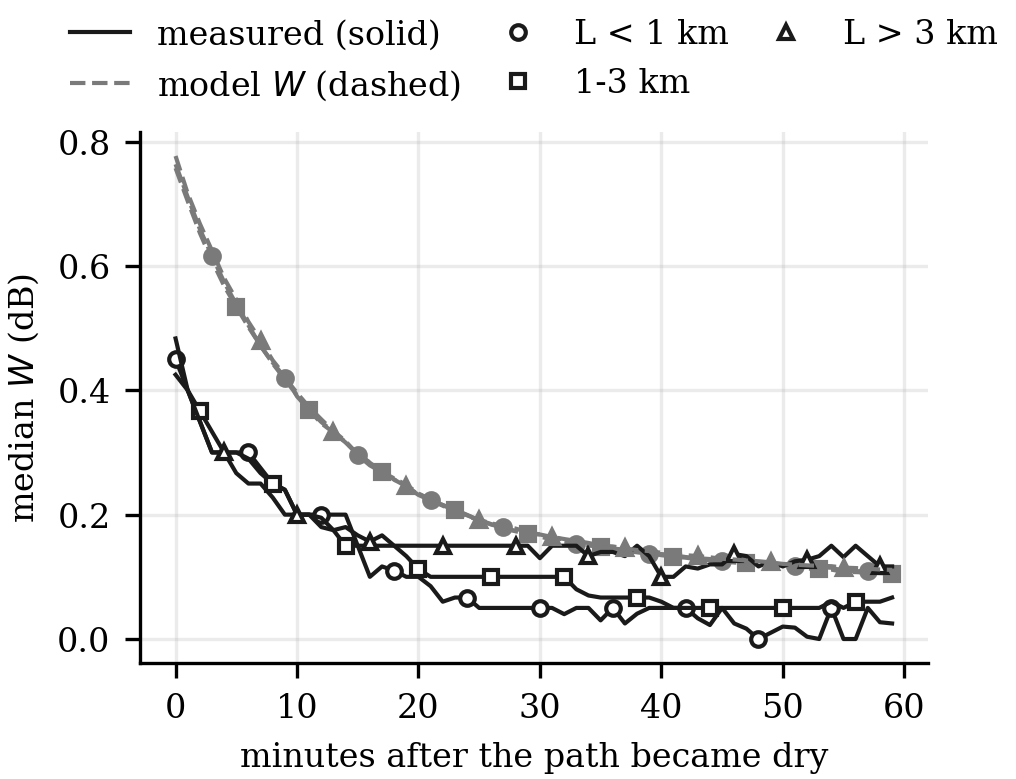
\includegraphics[width=\columnwidth]{v2_dry_path.png}
\caption{WAA measured after rain where no rain remains on the path (solid black) against the model (dashed grey), median
over 9\,081 windows of TRAIN and VAL, by length class (marker). The three classes agree. The model starts too high
(Sec.~\ref{sec:discussion}).}
\label{fig:drypath}
\end{figure}

\subsection{Comparison with other WAA models}
\label{sec:comparison}
All models were compared on the same task. Each receives only the corrected rain $R$, the length and the band, and
predicts the 5 min attenuation $A - c$ with the same events, baselines, offsets and path term $L\,\cband R$, and each was
fitted on TRAIN only. Three comparison models were frozen with our equation before TEST was read: no WAA, a constant WAA
while it rains, and a WAA without memory that has the same level curve as ours but no stores. The two published models were
added after TEST had been read, without any change to our equation, so their comparison is post-freeze. The Pastorek model
\cite{pastorek2022} is $W = C\,(1 - e^{-0.1 R^{\zeta}})$, with an upper limit $C$ per band and no memory. Its $\zeta$ acts
inside a saturating function and is not comparable with our $b$. The Schleiss model \cite{schleiss2013} rises toward
$W_{\max}$ while it rains and decays exponentially after, in the discrete form $W \leftarrow W + (W_{\max} - W)\,3\Delta
t/\twet$ of the open-source package pycomlink (version 0.6.0). That code uses the attenuation measured on the link itself,
which would give the model the answer, so a minute is wet here when $R > 0.1$ mm/h, and the dry step decays with its own
$\tdry$. Each published model was used in two versions. Version (a) keeps the default parameters and fits only $\cband$.
For the Schleiss model this requires a drying time that could not be checked in the paper, and it was set equal to the
wetting time (15 min), so version (a) is the pycomlink defaults with an assumed drying time, not the published model.
Version (b) fits all parameters on TRAIN with the same link factor as our equation, and its verdict is the one that
counts.

\begin{table*}[t]
\caption{Accuracy on TEST: RMSE of the 5 min attenuation in dB, and the paired difference to our equation (model minus
ours, 90\,\% interval from 1000 resampled sets of storms, the same draws for every model). Above zero means ours is better.
Ours: 0.695\iv{0.514}{0.803} dB for all links and 0.564\iv{0.436}{0.633} dB below 1 km.}
\label{tab:accuracy}
\begin{ruledtabular}
\begin{tabular}{lccc}
Model & RMSE & Minus ours, all & Minus ours, $L<1$ km\\
\hline
No WAA & 0.862 & $+0.167$\iv{+0.095}{+0.210} & $+0.275$\iv{+0.131}{+0.357}\\
Constant WAA & 0.760 & $+0.065$\iv{+0.047}{+0.075} & $+0.080$\iv{+0.047}{+0.099}\\
No memory & 0.727 & $+0.032$\iv{+0.019}{+0.049} & $+0.037$\iv{+0.021}{+0.058}\\
Schleiss (a) & 0.859 & $+0.164$\iv{+0.084}{+0.286} & $+0.200$\iv{+0.111}{+0.329}\\
Schleiss (b) & 0.703 & $+0.009$\iv{-0.010}{+0.039} & $+0.012$\iv{-0.009}{+0.044}\\
Pastorek (a) & 0.725 & $+0.031$\iv{+0.017}{+0.047} & $+0.027$\iv{+0.005}{+0.060}\\
Pastorek (b) & 0.720 & $+0.026$\iv{+0.015}{+0.038} & $+0.031$\iv{+0.017}{+0.046}\\
\end{tabular}
\end{ruledtabular}
\end{table*}

\begin{figure}[t]
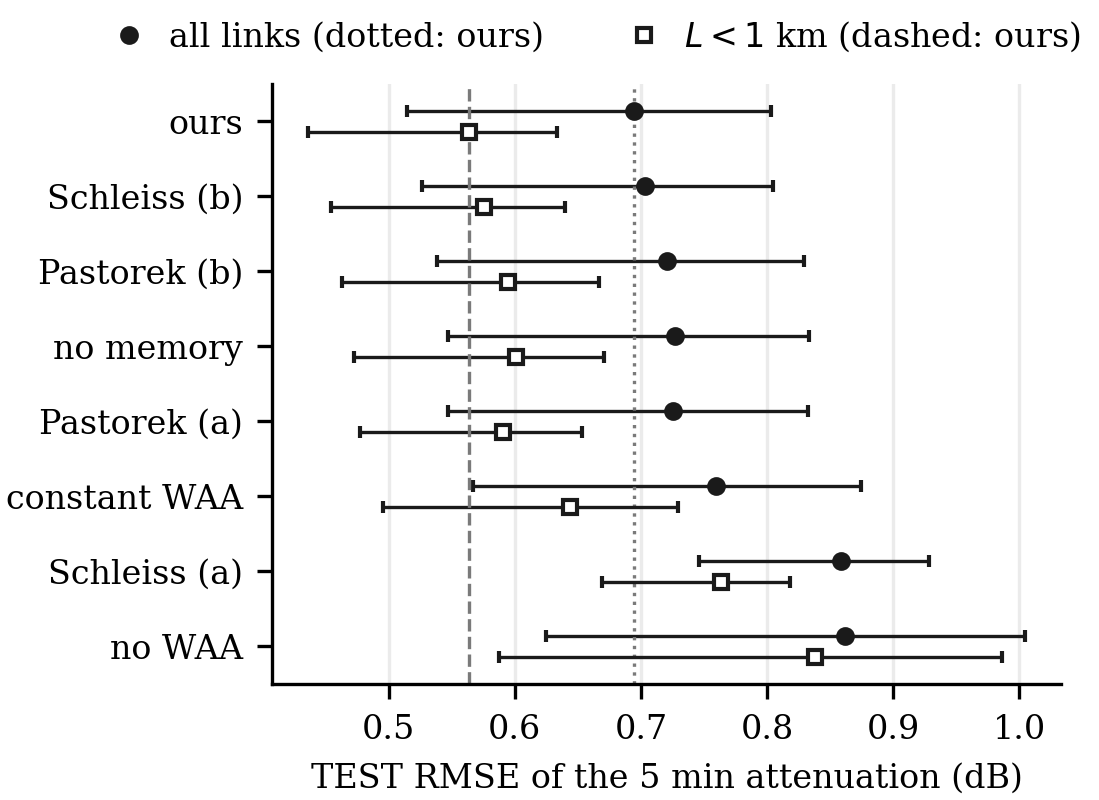
\includegraphics[width=\columnwidth]{v2_accuracy.png}
\caption{TEST RMSE of every model, all links (filled circles) and links below 1 km (open squares), with 90\,\% intervals.
The vertical lines mark our equation.}
\label{fig:accuracy}
\end{figure}

Table~\ref{tab:accuracy} and Fig.~\ref{fig:accuracy} give the accuracy. Our equation is better than every model whose
interval lies above zero, which is all of them except the refitted Schleiss model, with which it ties, on all links and on
links below 1 km. Accuracy alone, however, does not show that a model splits $A$ correctly into antenna and path. A model
can trade one part for the other and still fit the total. Table~\ref{tab:consistency} therefore compares each model with
four measurements that are independent of its fit: the slope and intercept of the length test, the WAA measured on dry
paths after rain, and the gauge timing. It also gives the correlation of each model's link factor with $L$, which should be
zero if the model's WAA does not depend on the length. This last check was added after the other numbers of
Table~\ref{tab:consistency} had been seen, because the refitted Pastorek model has a path loss of only 0.6 to 0.7 times
ours yet the measured slope. No pass rule was written for this table, and its numbers are reported as they came out.

\begin{table*}[t]
\caption{Physical consistency on TEST (post-freeze summary, nothing refitted). Length test: of the 8 eligible cells, the
number in which the model's own slope $s$ or intercept $I$ lies inside the model-free 90\,\% interval, and the median ratio
model / measured. Dry path: measured minus model WAA after the path became dry (1791 windows, median, positive means the
model holds too little water). The measured WAA is 0.35, 0.27 and 0.15 dB at 5, 10 and 20 min. $\rho(\alink, L)$: Spearman
correlation over the TRAIN links, 90\,\% link-bootstrap interval. Times: 1/e times of wetting and drying in min (Schleiss:
of its discrete step), against the gauge timing 2.6 and 10.3 min (VAL 2.0 and 8.8 min). Parameters: fitted global numbers,
with $\alink$ per link counted apart.}
\label{tab:consistency}
\footnotesize\setlength{\tabcolsep}{2pt}
\begin{ruledtabular}
\begin{tabular}{lccccccccc}
Model & $s$ in & $s$ ratio & $I$ in & $I$ ratio & Dry path 5/10/20 min (dB) & $\rho(\alink, L)$ & Wet/dry (min) & Param. & Identified\\
\hline
No WAA & 0 & 2.36 & 0 & 0.01 & $+0.35$ / $+0.27$ / $+0.15$ & -- & -- & 3 & no check\\
Constant WAA & 4 & 1.32 & 0 & 0.54 & $+0.35$ / $+0.27$ / $+0.15$ & $-0.60$\iv{-0.66}{-0.52} & 0 / 0 & 6 & no check\\
No memory & 7 & 0.97 & 6 & 0.81 & $+0.35$ / $+0.27$ / $+0.15$ & $+0.20$\iv{+0.08}{+0.32} & 0 / 0 & 12 & no check\\
Schleiss (a) & 5 & 0.65 & 2 & 1.38 & $-0.05$ / $+0.10$ / $+0.13$ & -- & 4.5 / 4.5 & 3 & no check\\
Schleiss (b) & 6 & 1.15 & 7 & 0.78 & $-0.24$ / $-0.25$ / $-0.18$ & $-0.45$\iv{-0.55}{-0.35} & 103 / 25 & 8 & no check\\
Pastorek (a) & 4 & 0.58 & 7 & 1.05 & $+0.33$ / $+0.25$ / $+0.15$ & -- & 0 / 0 & 3 & no check\\
Pastorek (b) & 7 & 0.97 & 6 & 0.82 & $+0.33$ / $+0.25$ / $+0.15$ & $+0.31$\iv{+0.18}{+0.42} & 0 / 0 & 7 & no check\\
Ours & 7 & 1.04 & 4 & 0.72 & $-0.19$ / $-0.15$ / $-0.11$ & $+0.09$\iv{-0.03}{+0.20} & 2.6 / 10.3 & 7 & 9 of 9 (fake data)\\
\end{tabular}
\end{ruledtabular}
\end{table*}

\begin{figure}[t]
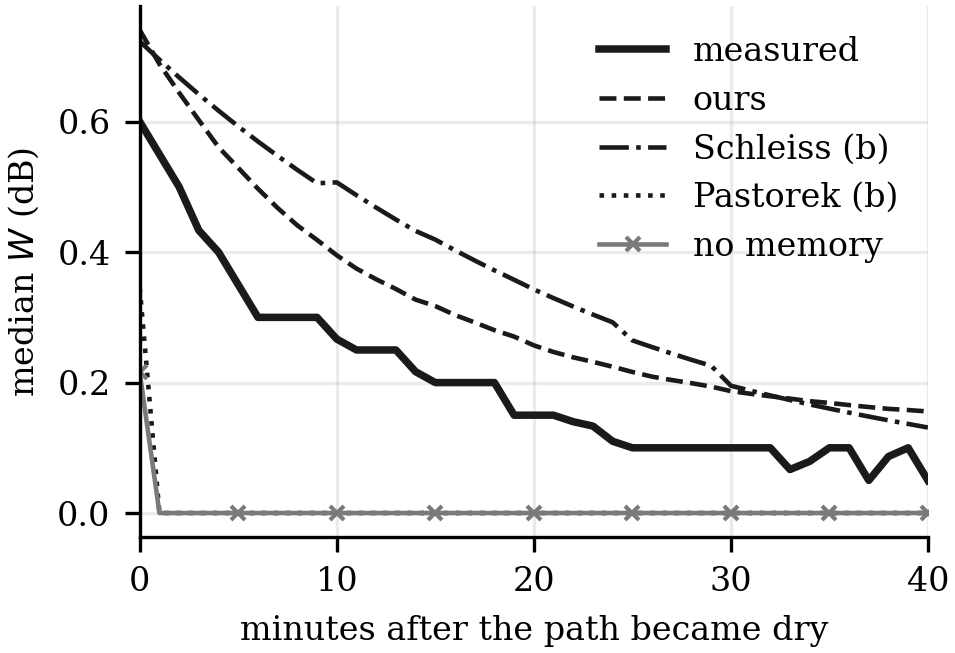
\includegraphics[width=\columnwidth]{v2_after_rain.png}
\caption{WAA on TEST after the path became dry: measured (thick solid) against our equation and the refitted published
models, median over 1791 windows on all lengths. The model without memory (grey crosses) and the Pastorek model fall to zero
when the rain stops.}
\label{fig:afterrain}
\end{figure}

The conclusion can be stated precisely. In accuracy our equation is better than or equal to every model, and it ties only
with the refitted Schleiss model. Of the models with a link factor, it is the only one whose link factor is independent of
the length. Its path loss agrees with the measured slope in 7 of 8 cells (median ratio 1.04). After rain no model agrees
with the measured WAA within its interval. Ours holds 0.11 to 0.19 dB too much water, the refitted Schleiss model 0.18 to
0.25 dB too much, and the models without memory 0.15 to 0.35 dB too little (Fig.~\ref{fig:afterrain}). Only the default
Schleiss version, with its assumed drying, has a smaller error at 5 and 10 min, at the price of a slope inside the measured
interval in only 5 of 8 cells. Our timing agrees with the gauges by construction, since it was measured with them, so it is
not independent evidence. Our equation is not the best on every measure. Its intercept agrees in only 4 of 8 cells, fewer
than the refitted Schleiss (7), the refitted Pastorek (6) and the model without memory (6), which is the failure discussed
in Sec.~\ref{sec:rules}. The refitted Schleiss model, which
ties in accuracy, reaches its fit with a path loss 1.7 to 1.8 times ours, a slope too high in heavy rain, a wetting time of
about 100 min and a drying time of about 25 min against the gauge times of 2.6 and 10.3 min, more water than measured after
rain, and a link factor that falls with the length. The refitted Pastorek model has a link factor that rises with the
length and no water at all after rain. The published models have neither fake-data recovery nor intervals.

\subsection{The test rules and the light-rain level}
\label{sec:rules}
TEST contains 18 storms, with 3\,355 link-events on known links and 1\,010 on 59 links that the model had never seen. After
the read, two errors were found in the evaluation code, not in the model: one storm with a radar-to-gauge ratio of zero and
three storms without a ratio had an undefined rain input. Both received the fallback $g_e = 1$ that the rule already
specified, and the numbers before and after the fix were recorded. Table~\ref{tab:rules} gives the five rules, written
before the read, for the model frozen for the test.

\begin{table*}[t]
\caption{The five test rules, written before TEST was read, and the results for the frozen model.}
\label{tab:rules}
\begin{tabularx}{\textwidth}{lLl}
\toprule
Rule & Result & Verdict\\
\midrule
P1 length test & 4 of 8 cells agree (6 needed): slopes 7 of 8, intercepts 4 of 8 & fail\\
P2 beats simpler models & 0.692 dB against 0.862, 0.760, 0.727; below 1 km 0.562 against 0.838, 0.644, 0.601 & pass\\
P3 equal WAA by length & dry-path error, long minus short, $-0.04$\iv{-0.15}{+0.04} dB & pass\\
P4 no class out of line & TEST / VAL ratio 1.12, each class within 5\,\% of it & pass\\
P5 new links & error 1.07 times that on known links (limit 1.20) & pass\\
\bottomrule
\end{tabularx}
\end{table*}

The failed rule locates the limit of the equation. The slopes, which measure the rain on the path, agree in 7 of 8 cells.
The intercepts, which measure the WAA, disagree in light rain (0.5 to 2 mm/h), where the test storms had 1.35 to 1.55 dB
against 0.83 to 1.11 dB in the equation. The WAA level in light rain therefore varies between storms more than the equation
describes. The failure is not a dependence on length, which P3 tested and passed.

The equation frozen for the test described $F$ by its free curve. The closed form had been fitted before the freeze but
was not the frozen version. After the test it was evaluated on the same data without refitting, under a rule written before
the evaluation: adopted only if it gives the same five verdicts and its error lies within $\pm 0.01$ dB of the free curve.
Both held, with the same verdicts and a difference of $+0.0025$ dB ($-0.0065$ to $+0.0085$), so the closed form is the
written form of $F$ (Fig.~\ref{fig:model}).

% =====================================================================================================================
\section{Discussion}
\label{sec:discussion}

The tie with the refitted Schleiss model is not an equivalence. Two models can predict the total attenuation equally well
while they split it differently between the antennas and the path, because during most of a storm both parts rise and fall
with the same rain. The split is visible only where the two parts behave differently, along the length and after the rain,
and there the two models disagree. The Schleiss fit puts 1.7 to 1.8 times more loss on the path and compensates on short
links with a link factor that falls with length. In effect its WAA depends on the length, which our three tests
of Sec.~\ref{sec:indep} do not find in the data. Its
wetting time of about 100 min also contradicts the gauge timing, which shows the film forming within 2 to 3 min. Equal
accuracy with an unphysical split would carry the error into Part 2, where the path law is learned after the WAA is
removed.

The one failed test rule concerns the WAA level in light rain. On the test storms the intercept at 0.5 to 2 mm/h was about
0.4 to 0.6 dB higher than the final equation, while the slope agreed. A single curve $F(R)$ cannot carry a level that
depends on the storm, for example on how long it rained before or on the drop sizes of light rain, but neither cause was
tested. The refitted Schleiss and Pastorek models and the model without memory match this level more often (6 or 7 of 8
intercepts), but they do so with a link factor that changes with the length or with no water after the rain, so their
better intercept does not come with a better split. Why our equation sits low in light rain is not known. The slow store,
which is not identified, is one candidate, because it sets how much of the level is reached after a given time of steady
rain.

After the rain our equation holds about 0.25 dB more water than measured at the moment the path becomes dry, and about
0.5 dB after heavy rain (Fig.~\ref{fig:drypath}). The causes were tested one by one. The measured decay rate is 0.87 times
that of the model (interval 0.70 to 1.06), so the drying speed is consistent, and the error lies in the amount of water at
the end of the rain. It is not caused by the radar timing, and the model is not too high during heavy rain. The error is
larger after heavier rain and in drier air. Water running off the radome, which has been seen in the laboratory
\cite{tiede2025}, would explain this, but this work cannot confirm it. A version with a free drying time of 3.7 min removes
the misfit, but it was not adopted. With so fast a drying the antenna part follows the rain almost as quickly as the path
part, the two can no longer be separated, and the path loss halves with an interval reaching zero in every band. The
3.7 min is an effective time for the 5 min radar input, not the drying time measured with the gauges. The faster drying
therefore stays outside the equation, and so does the wind, whose apparent effect on the drying (Spearman $-0.76$ over 17
storms) disappeared once the preceding rain was held fixed.

Dew wets the same antennas without rain. On 125 humid link-nights the attenuation rose by a median of 1.7 dB for about 4 h,
and links with a larger $\alink$ also had more dew (Spearman $+0.26$). Dew is therefore a real WAA, but it is not driven by
rain and was left out of the equation on purpose.

The error budget shows where the remaining error lies. On TEST, 61\,\% of the squared error occurs during rain within storms,
8\,\% is the difference between storms (the rain reference), 6\,\% falls in the hour after rain and 25\,\% in dry minutes.
On VAL the shares within storms and after rain are 65\,\% and 2\,\%. The after-rain misfit is thus a small part of the error.
A likely cause of the large part is that the radar resolves rain more coarsely (5 min, 2 km) than a link does, but this has
not been tested.

The path loss of the equation is linear in $R$, $P = \cband R$. A power law fitted to the free points of $P$ gave an
exponent of 0.97 with a quadratic term of zero, and the ITU-R P.838 exponents at 28 to 38 GHz are 0.86 to 0.92
\cite{itu838}, so both describe a nearly linear loss in this range. Its size is 0.52 to 0.74 times the ITU-R value. Whether
this is a remaining scale error of the radar rain or an effect of uneven rain along the path, which is what $f(L,\Rb,Z)$
in Part 2 is meant to capture, cannot be decided here.

Table~\ref{tab:boxes} states what the model claims. Box A is in the equation, with identified numbers. Box B is identified
but kept outside, because adding it would unbind another number. Box C is seen but not explained.

\begin{table}[t]
\caption{What the model claims.}
\label{tab:boxes}
\begin{tabularx}{\columnwidth}{lL}
\toprule
Box & Content\\
\midrule
A, in the equation & the level rising about as $\sqrt{R}$, one shape for all bands, the fast store (2.6 and 10.3 min), the slow store as a structure, $P = \cband R$, the band levels, the link factor, $W$ independent of $L$\\
B, outside & faster drying with wind, the end-of-rain level (larger after heavy rain and in dry air), dew\\
C, unexplained & the numbers of the slow store, the cause of the link factor, $F$ above 10 mm/h, $P$ below 1 mm/h, the WAA level in light rain between storms\\
\bottomrule
\end{tabularx}
\end{table}

% =====================================================================================================================
\section{Conclusions}
\label{sec:conclusions}

A dynamic wet antenna law was identified from the OpenMRG links without subtracting any rain law. The antenna and the
path were separated by the link length and by the dry paths after rain, and the result is a fast and a slow store whose
target grows about as the square root of the rain rate, with a wetting time of 2.6 min, a drying time of 10.3 min, and a
path loss linear in the rain. On held-out storms, read once after a hashed freeze, it predicts the attenuation better than
or as well as every other model tested, and of the models with a link factor it is the only one whose link factor does not change with the link length.
Its limit is the WAA level in light rain, which varies between storms. The next step is to remove the WAA with this
equation and test whether the rain estimated from the links agrees better with the gauges, which needs its own written
plan and a decision about TEST, which has already been read once. Part 2 will then learn the path law $f(L,\Rb,Z)$ with
the WAA removed by the frozen equation.

% =====================================================================================================================
\appendix

\section{The baseline}
\label{app:baseline}
For each event and sub-link the baseline is one constant. The 24 h before the event start are taken (48 h if less than 1 h
of dry data remains), only the 5 min slots that radar and gauges mark as dry and that start at least 1 h after the last rain
are kept, and the baseline is the median attenuation over them. The rule of 1 h excludes the drying after earlier rain.
Links with a large daily cycle of the dry level or with erratic behaviour are flagged and excluded. The method was tested
where the truth is known by placing fake events inside dry periods, where the correct WAA is zero. For 6 h events the
median error was 0.00 dB, with 10th and 90th percentiles of $-0.21$ and $+0.22$ dB, so the error has no bias and averages
out over many events. Each sub-link keeps its own measured error, and sub-links with an error above 0.3 dB are excluded. A
second test checked that the baseline does not absorb the drying after rain. One hour after real rain the level was
0.04 dB above that of a dry control, and the difference fell to zero within 12 h. The same test showed the rises on humid
nights that are attributed to dew.

\section{Decisions}
\label{app:decisions}
Table~\ref{tab:decisions} lists the decisions that changed the course of the work, with their dates and reasons. Decisions
marked as deviations override a written rule, and each is stated openly.

\begin{table*}[t]
\caption{The dated decisions of Part 1.}
\label{tab:decisions}
\begin{tabularx}{\textwidth}{lLL}
\toprule
Date (2026) & Decision & Reason\\
\midrule
7 Oct & Baseline frozen (median of the dry 24 h) & unbiased on fake events, does not absorb the drying\\
13 Oct & Drying tails closed, restart as system identification of whole events & tails wait or rise, most of a tail passes while it rains nearby, no law identified (Appendix~\ref{app:side})\\
17 Oct & Radar divided by the event's radar-to-gauge factor & VAL length test 1 of 8 cells with the raw radar, 5 of 6 with the factor\\
18 Oct & Two-store model with gauge timing kept, a more flexible slow store dropped (deviation) & its slow store was not identified, gain 0.0005 dB on VAL; decided after seeing VAL\\
19 Oct & Closed form of $F$ not adopted before the test & failed the length test at exactly 4 of 6 cells against a written 0.6667\\
19 Oct & Faster drying (3.7 min) kept outside the equation (deviation) & passed its rules but unbound the path loss\\
19 Oct & Freeze, hashes committed, TEST read once & protocol\\
19 Oct & Closed form of $F$ adopted after the test & same five verdicts, difference within $\pm 0.01$ dB, rule written first\\
28 Oct & Schleiss (b) searched on a coarse grid, then refined & first run stopped by low memory, changed before any result\\
2 Nov & Link factor against $L$ added to Table~\ref{tab:consistency} & added after its other numbers were seen\\
\bottomrule
\end{tabularx}
\end{table*}

\section{Side roads}
\label{app:side}
The first phase studied drying tails, the stretches of $A$ after rain. From 20\,355 extracted tails a frozen set of 429
training tails was selected by rules that never looked at the decay. A simulator calibrated to the real tails showed that
fitting tails one at a time cannot identify a drying law, that fitting all tails together with a shared law can, and that
SINDy \cite{brunton2016} applied directly to the noisy, quantised tails cannot. On the real tails no drying law was
identified, because about one tail in five stays flat or rises after the rain, most of a tail passes while it still rains
nearby, and the fast first drop does not grow with the path length. The tail was the wrong object, and the phase was closed
on 13 October.

The system identification that replaced it fitted a ladder of models of growing complexity to whole events, each first
checked on fake data. A flexible rung in which the wetting and drying could be any function of rain and stored water, to be
named afterwards by sparse regression or PySR, was not identified on real data. Factors per event, fitted to absorb the
differences between storms, failed their fake check on light events. A slow store with separate wetting and drying times
passed its rule but its numbers were not identified (Appendix~\ref{app:decisions}). A wind-dependent drying improved the
fit but failed the rules that require stable numbers, and a drying that depends on the preceding rain had no effect. A
rain-rate dependent correction of the radar was not justified. Pairs of links on a common path, which would measure $W$
directly, were too few to test (4 pairs).

\section{Uncertainty and identifiability}
\label{app:uncertainty}
All fits minimise a Huber loss of the 5 min residuals (threshold 0.3 dB), which limits the effect of outliers, plus a prior
on $\ln\alink$. Intervals of the equation's numbers are the 5th and 95th percentiles of 40 refits on sets of TRAIN events
drawn with replacement, each refit started cold. Resampling whole events keeps the correlation between the minutes and the
links of one storm. Profile intervals, which vary one number and refit the others, were 1 to 13 times narrower than the
bootstrap intervals for most numbers, so the event-to-event variation of the rain reference dominates the uncertainty. A
number counts as identified if it is recovered within 20\,\% on three fake datasets generated from the fitted model with
realistic noise on the real links and rain, and if its interval does not reach a search bound. Test intervals are the 5th
and 95th percentiles of 1000 resampled sets of TEST storms, with the same draws for every model so that differences are
paired. The fixed time constants come from warm-started refits of the gauge-input fit, and their intervals may be too
narrow.

\section{Full TEST tables}
\label{app:tables}
Table~\ref{tab:fullrmse} gives the TEST error by length class. Table~\ref{tab:cells} gives the eight cells of the length test
with the measured intervals and the values of each model. The full tables, including the links never fitted, are in the
step reports of the project.

\begin{table}[t]
\caption{TEST RMSE (dB) by length class. 90\,\% intervals are in the step reports.}
\label{tab:fullrmse}
\begin{ruledtabular}
\begin{tabular}{lcccc}
Model & $L<1$ km & 1--3 km & $L>3$ km & All\\
\hline
Ours & 0.564 & 0.684 & 0.780 & 0.695\\
No WAA & 0.838 & 0.850 & 0.895 & 0.862\\
Constant WAA & 0.644 & 0.750 & 0.837 & 0.760\\
No memory & 0.601 & 0.715 & 0.812 & 0.727\\
Schleiss (a) & 0.763 & 0.845 & 0.934 & 0.859\\
Schleiss (b) & 0.576 & 0.693 & 0.787 & 0.703\\
Pastorek (a) & 0.590 & 0.706 & 0.826 & 0.725\\
Pastorek (b) & 0.595 & 0.709 & 0.805 & 0.720\\
\end{tabular}
\end{ruledtabular}
\end{table}

\begin{table*}[t]
\caption{The eight eligible cells of the TEST length test. Measured: slope $s$ (dB/km) and intercept $I$ (dB) with 90\,\%
intervals. Models: their own slope and intercept on the same values. Values inside the measured interval are marked with an
asterisk.}
\label{tab:cells}
\begin{ruledtabular}
\begin{tabular}{llcccccccc}
Band & Class & Measured & No WAA & Const. & No mem. & Schleiss (b) & Pastorek (b) & Ours\\
\hline
\multicolumn{9}{l}{Slope $s$ (dB/km)}\\
28 GHz & 0.5--1 & 0.037\iv{0.014}{0.077} & 0.210 & 0.046* & 0.098 & 0.042* & 0.103 & 0.096\\
28 GHz & 1--2 & 0.164\iv{0.086}{0.234} & 0.374 & 0.179* & 0.143* & 0.188* & 0.153* & 0.168*\\
28 GHz & 2--5 & 0.313\iv{0.205}{0.439} & 0.708 & 0.453 & 0.273* & 0.396* & 0.266* & 0.295*\\
28 GHz & 5--10 & 0.603\iv{0.513}{0.863} & 1.537 & 1.083 & 0.588* & 0.984 & 0.552* & 0.643*\\
38 GHz & 0.5--1 & 0.150\iv{0.082}{0.221} & 0.365 & 0.107* & 0.201* & 0.124* & 0.200* & 0.178*\\
38 GHz & 1--2 & 0.332\iv{0.203}{0.455} & 0.669 & 0.357* & 0.322* & 0.324* & 0.333* & 0.311*\\
38 GHz & 2--5 & 0.598\iv{0.296}{0.787} & 1.289 & 0.826 & 0.513* & 0.689* & 0.503* & 0.522*\\
38 GHz & 5--10 & 0.850\iv{0.121}{1.570} & 2.839 & 2.045 & 1.129* & 1.721 & 1.085* & 1.187*\\
\multicolumn{9}{l}{Intercept $I$ (dB)}\\
28 GHz & 0.5--1 & 1.35\iv{0.99}{1.52} & 0.00 & 0.90 & 0.88 & 1.14* & 0.87 & 0.80\\
28 GHz & 1--2 & 1.43\iv{1.15}{1.71} & 0.02 & 0.90 & 1.20* & 1.11 & 1.22* & 1.05\\
28 GHz & 2--5 & 1.79\iv{1.22}{2.13} & 0.07 & 0.90 & 1.82* & 1.38* & 1.71* & 1.50*\\
28 GHz & 5--10 & 2.60\iv{1.11}{3.47} & 0.13 & 0.99 & 2.44* & 1.46* & 2.47* & 2.11*\\
38 GHz & 0.5--1 & 1.44\iv{1.11}{1.60} & 0.01 & 0.93 & 0.93 & 1.18* & 0.93 & 0.87\\
38 GHz & 1--2 & 1.55\iv{1.20}{1.79} & $-0.01$ & 0.91 & 1.21* & 1.23* & 1.24* & 1.09\\
38 GHz & 2--5 & 2.00\iv{1.54}{2.31} & 0.04 & 0.95 & 2.00* & 1.57* & 1.86* & 1.66*\\
38 GHz & 5--10 & 3.42\iv{1.01}{4.90} & $-0.01$ & 0.89 & 2.64* & 1.68* & 2.60* & 2.28*\\
\end{tabular}
\end{ruledtabular}
\end{table*}

% =====================================================================================================================
\begin{thebibliography}{99}
\bibitem{messer2006} H. Messer, A. Zinevich, and P. Alpert, ``Environmental monitoring by wireless communication
networks,'' \emph{Science} \textbf{312}, 713 (2006). \url{https://doi.org/10.1126/science.1120034}
\bibitem{itu838} ITU-R, ``Specific attenuation model for rain for use in prediction methods,'' Recommendation ITU-R P.838-3
(2005).
\bibitem{leijnse2008} H. Leijnse, R. Uijlenhoet, and J. N. M. Stricker, ``Microwave link rainfall estimation: effects of link
length and frequency, temporal sampling, power resolution, and wet antenna attenuation,'' \emph{Adv. Water Resour.}
\textbf{31}, 1481--1493 (2008). \url{https://doi.org/10.1016/j.advwatres.2008.03.004}
\bibitem{schleiss2013} M. Schleiss, J. Rieckermann, and A. Berne, ``Quantification and modeling of wet-antenna attenuation for
commercial microwave links,'' \emph{IEEE Geosci. Remote Sens. Lett.} \textbf{10}, 1195--1199 (2013).
\url{https://doi.org/10.1109/LGRS.2012.2236074}
\bibitem{pastorek2022} J. Pastorek, M. Fencl, J. Rieckermann, and V. Bare\v{s}, ``Precipitation estimates from commercial
microwave links: practical approaches to wet-antenna correction,'' \emph{IEEE Trans. Geosci. Remote Sens.} \textbf{60},
1--9 (2022). \url{https://doi.org/10.1109/TGRS.2021.3110004}
\bibitem{tiede2023} J. Tiede, C. Chwala, and U. Siart, ``New insights into the dynamics of wet antenna attenuation based on
in situ estimations provided by the dedicated field experiment ATTRRA2,'' \emph{IEEE Geosci. Remote Sens. Lett.}
\textbf{20} (2023). \url{https://doi.org/10.1109/LGRS.2023.3320755}
\bibitem{tiede2025} J. Tiede, C. Chwala, U. Siart, and T. Eibert, ``Frequency-dependent variations of the antenna reflection
coefficient due to different wetness conditions on the antenna radome,'' \emph{Adv. Radio Sci.} \textbf{23}, 13--19 (2025).
\url{https://doi.org/10.5194/ars-23-13-2025}
\bibitem{openmrg} J. C. M. Andersson, J. Olsson, R. van de Beek, and J. Hansryd, ``OpenMRG: Open data from Microwave links,
Radar, and Gauges for rainfall quantification in Gothenburg, Sweden,'' \emph{Earth Syst. Sci. Data} \textbf{14}, 5411--5426
(2022). \url{https://doi.org/10.5194/essd-14-5411-2022}
\bibitem{cranmer2023} M. Cranmer, ``Interpretable machine learning for science with PySR and SymbolicRegression.jl,''
arXiv:2305.01582 (2023).
\bibitem{brunton2016} S. L. Brunton, J. L. Proctor, and J. N. Kutz, ``Discovering governing equations from data by sparse
identification of nonlinear dynamical systems,'' \emph{Proc. Natl. Acad. Sci. USA} \textbf{113}, 3932--3937 (2016).
\url{https://doi.org/10.1073/pnas.1517384113}
\end{thebibliography}

\end{document}
